% =============================================================================
%  RK-PINNs for Track Extrapolation — Motivation & Literature
%  Author: G. Scriven (LHCb, Nikhef)
%  Date:   March 2026
% =============================================================================
\documentclass[aspectratio=169, 11pt]{beamer}

% ---- Theme & Colours --------------------------------------------------------
\usetheme{Madrid}
\usecolortheme{default}

\definecolor{lhcbblue}{HTML}{1F77B4}
\definecolor{nngreen}{HTML}{2CA02C}
\definecolor{rkorange}{HTML}{FF7F0E}
\definecolor{rk4red}{HTML}{D62728}
\definecolor{lightgray}{HTML}{F0F0F0}
\definecolor{darkgray}{HTML}{404040}
\definecolor{physpurple}{HTML}{9467BD}

\setbeamercolor{title}{fg=white, bg=lhcbblue}
\setbeamercolor{frametitle}{fg=white, bg=lhcbblue}
\setbeamercolor{structure}{fg=lhcbblue}
\setbeamercolor{block title}{bg=lhcbblue!20, fg=black}
\setbeamercolor{block body}{bg=lhcbblue!5}
\setbeamercolor{block title alerted}{bg=rk4red!20, fg=black}
\setbeamercolor{block body alerted}{bg=rk4red!5}
\setbeamercolor{block title example}{bg=nngreen!20, fg=black}
\setbeamercolor{block body example}{bg=nngreen!5}
\setbeamertemplate{navigation symbols}{}
\setbeamertemplate{footline}[frame number]

% ---- Packages ---------------------------------------------------------------
\usepackage[utf8]{inputenc}
\usepackage[T1]{fontenc}
\usepackage{lmodern}
\usepackage{amsmath,amssymb}
\usepackage{booktabs}
\usepackage{array}
\usepackage{colortbl}
\usepackage{xcolor}
\usepackage{tikz}
\usetikzlibrary{arrows.meta, positioning, shapes.geometric, calc,
                decorations.pathreplacing, fit}
\usepackage{hyperref}
\usepackage{bm}
\usepackage{multicol}
\usepackage{pifont}
\newcommand{\vb}[1]{\bm{#1}}

% =============================================================================
\title[RK-PINNs for Track Extrapolation]{%
  \textbf{Runge--Kutta Physics-Informed Neural Networks}\\[4pt]
  \large Motivation from the LHCb Track Extrapolation Problem}

\author{G.~Scriven}
\institute{Maastricht University\quad$\cdot$\quad UHasselt\quad$\cdot$\quad LHCb}
\date{March 2026}

\begin{document}

% =============================================================================
\begin{frame}[plain]
  \titlepage
\end{frame}

% =============================================================================
\begin{frame}{Outline}
  \tableofcontents
\end{frame}

% =============================================================================
\section{The Physics Problem}
% =============================================================================

\begin{frame}{Track Extrapolation in LHCb}
  \begin{columns}[T]
    \column{0.58\textwidth}
    Charged particles traverse the LHCb dipole magnet and are bent by the Lorentz force.

    \medskip
    \textbf{Equations of motion} (4 coupled ODEs, $z$ as ind.\ variable):
    {\footnotesize
    \begin{align*}
      \frac{dx}{dz} &= t_x, \quad \frac{dy}{dz} = t_y \\[3pt]
      \frac{dt_x}{dz} &= \kappa N \bigl[ t_x t_y B_x - (1{+}t_x^2)B_y + t_y B_z \bigr] \\[2pt]
      \frac{dt_y}{dz} &= \kappa N \bigl[ (1{+}t_y^2)B_x - t_x t_y B_y - t_x B_z \bigr]
    \end{align*}
    }%
    $\kappa = (q/p)\cdot c_\text{light}$, \quad $N = \sqrt{1+t_x^2+t_y^2}$

    \column{0.39\textwidth}
    \begin{block}{The mapping}
      {\small $f: (x_0, y_0, t_{x,0}, t_{y,0}, q/p, \Delta z)
        \to (x_f, y_f, t_{x,f}, t_{y,f})$}
      \\\centering\scriptsize 6D input $\to$ 4D output
    \end{block}

    \begin{alertblock}{Challenge}
      \begin{itemize}
        \item $\vb{B}(x,y,z)$ is a \textbf{3D tabulated} field
        \item Non-uniform, non-analytic
        \item $81 \times 81 \times 146$ grid
        \item $\Delta z$ up to 8000\,mm
      \end{itemize}
    \end{alertblock}
  \end{columns}
\end{frame}

% -----------------------------------------------------------------------------
\begin{frame}{The LHCb Magnetic Field}
  \begin{columns}[T]
    \column{0.54\textwidth}
    \textbf{Field characteristics} (from \texttt{twodip.rtf}):
    \begin{itemize}\setlength{\itemsep}{1pt}
      \item Dominant: $B_y$ (vertical, bends in $xz$-plane)
      \item Peak $B_y = -1.02$\,T at $z \approx 5250$\,mm
      \item FWHM $\approx 3400$\,mm; active: $z \in [2000, 9400]$
      \item $B_x, B_z$: fringe fields (${\sim}$10\% of $B_y$)
    \end{itemize}

    \smallskip
    {\small\textbf{Gaussian approx.}\ ($B_y \!\approx\! B_0 e^{-(z-z_c)^2/2\sigma^2}$):}
    \begin{itemize}\setlength{\itemsep}{1pt}
      \item RMS error: 20.8\,mT (3.2\%)
      \item \textcolor{rk4red}{\textbf{Not suitable}} for precision training
    \end{itemize}

    \column{0.43\textwidth}
    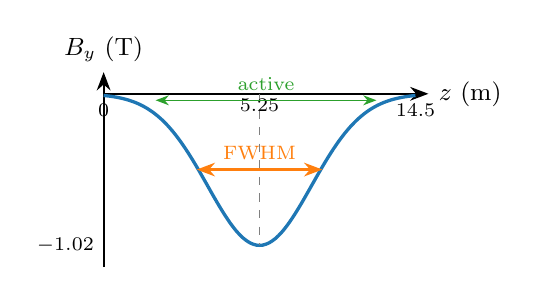
\begin{tikzpicture}[scale=0.55]
      % B_y(z) profile sketch
      \draw[-Stealth, thick] (0,0) -- (7.5,0) node[right] {\small $z$ (m)};
      \draw[-Stealth, thick] (0,-4) -- (0,0.5) node[above] {\small $B_y$ (T)};
      % Gaussian-ish curve
      \draw[lhcbblue, very thick, smooth] plot[domain=0:7.2, samples=50]
        (\x, {-3.5*exp(-0.5*((\x-3.6)/1.2)^2)});
      % Peak label
      \draw[dashed, gray] (3.6,0) -- (3.6,-3.5);
      \node[below, font=\scriptsize] at (3.6,0.1) {5.25};
      \node[left, font=\scriptsize] at (0,-3.5) {$-1.02$};
      % FWHM
      \draw[Stealth-Stealth, rkorange, thick] (2.15,-1.75) -- (5.05,-1.75);
      \node[above, font=\scriptsize, rkorange] at (3.6,-1.75) {FWHM};
      % Active region
      \draw[Stealth-Stealth, nngreen] (1.2,-0.15) -- (6.3,-0.15);
      \node[above, font=\scriptsize, nngreen] at (3.75,-0.15) {active};
      % z labels
      \node[below, font=\scriptsize] at (0,0) {0};
      \node[below, font=\scriptsize] at (7.2,0) {14.5};
    \end{tikzpicture}

    \medskip
    \begin{exampleblock}{Key insight}
      \footnotesize Field is \textbf{smooth} and \textbf{slowly varying}---ideal for numerical integration.
    \end{exampleblock}
  \end{columns}
\end{frame}

% =============================================================================
\section{The Speed Problem}
% =============================================================================

\begin{frame}{Why Speed Matters}
  \begin{columns}[T]
    \column{0.55\textwidth}
    \textbf{LHCb Upgrade~II (Run~5+):}
    \begin{itemize}\setlength{\itemsep}{2pt}
      \item 40\,MHz bunch crossing rate
      \item Full software trigger (no L0 hardware)
      \item Track extrapolation: $\mathcal{O}(10^3)$/event
    \end{itemize}

    \smallskip
    \textbf{Current C++ RK4 extrapolator:}
    \begin{itemize}\setlength{\itemsep}{2pt}
      \item CashKarp scheme (6-stage adaptive)
      \item Per sub-step: \textbf{6 field lookups} + interpolation
      \item $\Delta z{=}8000$\,mm, step${=}$5\,mm:
            $\sim$1600$\times$6 = \textbf{9600 field evals}
      \item Total: \textbf{7.50\,$\mu$s per call}
    \end{itemize}

    \column{0.42\textwidth}
    \begin{block}{Cost breakdown}
      \centering
      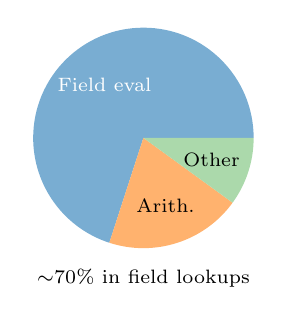
\begin{tikzpicture}[scale=0.7]
        \fill[lhcbblue!60] (0,0) -- (0:2) arc (0:252:2) -- cycle;
        \fill[rkorange!60] (0,0) -- (252:2) arc (252:324:2) -- cycle;
        \fill[nngreen!40] (0,0) -- (324:2) arc (324:360:2) -- cycle;
        \node[font=\scriptsize, white] at (126:1.2) {Field eval};
        \node[font=\scriptsize] at (288:1.3) {Arith.};
        \node[font=\scriptsize] at (342:1.3) {Other};
        \node[below, font=\scriptsize] at (0,-2.2) {$\sim$70\% in field lookups};
      \end{tikzpicture}
    \end{block}
    \begin{alertblock}{Bottleneck}
      \small Field interpolation dominates. An NN replaces \textbf{all 9600 lookups} with one forward pass.
    \end{alertblock}
  \end{columns}
\end{frame}

% -----------------------------------------------------------------------------
\begin{frame}{Three Architecture Approaches}
  \begin{columns}[T]
    \column{0.32\textwidth}
    \begin{block}{\textcolor{nngreen}{MLP} --- Black-box}
      Direct function approximation:
      \[
        \hat{\vb{y}} = \text{MLP}(\vb{x}_0, q/p, \Delta z)
      \]
      \begin{itemize}
        \item No physics knowledge
        \item Fastest inference
        \item Needs abundant data
      \end{itemize}
    \end{block}

    \column{0.32\textwidth}
    \begin{block}{\textcolor{rkorange}{PINN} --- Physics loss}
      MLP + physics regularisation:
      \[
        \mathcal{L} = \mathcal{L}_\text{data} + \lambda\,\mathcal{L}_\text{PDE}
      \]
      \begin{itemize}
        \item ODE residual as penalty
        \item Needs differentiable field
        \item Slower training (AD)
      \end{itemize}
    \end{block}

    \column{0.32\textwidth}
    \begin{block}{\textcolor{lhcbblue}{RK-PINN} --- Structured}
      RK4-inspired multi-stage:
      \[
        \hat{\vb{y}} = \vb{y}_0 + \sum_k w_k\,\Delta\vb{s}_k
      \]
      \begin{itemize}
        \item Physics in architecture
        \item IC by construction
        \item Learnable RK weights
      \end{itemize}
    \end{block}
  \end{columns}

  \bigskip
  \centering
  \fbox{\parbox{0.82\textwidth}{\centering
    Each approach represents a different level of physics integration: \\
    \textbf{none} (MLP) $\to$ \textbf{soft constraint} (PINN) $\to$ \textbf{structural bias} (RK-PINN)
  }}
\end{frame}

% -----------------------------------------------------------------------------
\begin{frame}{Benchmark Results: MLPs Win on Speed}
  \centering
  \begin{tabular}{llrrrr}
    \toprule
    \textbf{Model} & \textbf{Type} & \textbf{Params} & \textbf{Time ($\mu$s)} & \textbf{Speedup} & \textbf{Error} \\
    \midrule
    \rowcolor{nngreen!10} mlp\_single & MLP & 18k & \textbf{0.83} & \textbf{9.0$\times$} & 65\,$\mu$m \\
    \rowcolor{nngreen!10} mlp\_tiny & MLP & 4.9k & 1.12 & 6.7$\times$ & 53\,$\mu$m \\
    mlp\_small & MLP & 17.9k & 1.22 & 6.1$\times$ & 53\,$\mu$m \\
    mlp\_shallow & MLP & 100k & 1.28 & 5.9$\times$ & 33\,$\mu$m \\
    mlp\_medium & MLP & 101k & 2.17 & 3.5$\times$ & 37\,$\mu$m \\
    \midrule
    pinn\_medium & PINN & 101k & 2.46 & 3.0$\times$ & \textcolor{rk4red}{593\,mm} \\
    rkpinn\_tiny & RK-PINN & --- & 3.91 & 1.9$\times$ & \textcolor{rk4red}{$>10^5$\,$\mu$m} \\
    rkpinn\_medium & RK-PINN & 202k & 5.59 & 1.3$\times$ & \textcolor{rk4red}{2\,km} \\
    \midrule
    Kisel & C++ & --- & 1.50 & 5.0$\times$ & 39.8\,mm \\
    Reference RK4 & C++ & --- & 7.50 & 1.0$\times$ & 0 (ref.) \\
    \bottomrule
  \end{tabular}

  \bigskip
  \textcolor{rk4red}{\textbf{Physics-informed models were slower AND catastrophically wrong.}} \\
  \textcolor{lhcbblue}{But was the failure fundamental, or fixable?}
\end{frame}

% =============================================================================
\section{Why PINNs Failed}
% =============================================================================

\begin{frame}{PINN Failure --- Root Cause Analysis}
  \begin{columns}[T]
    \column{0.48\textwidth}
    \textbf{Bug:} \texttt{forward()} hardcoded \texttt{z\_frac = 1.0}
    \begin{enumerate}\setlength{\itemsep}{1pt}
      \item Network only trained at \textbf{one} $z$-value
      \item Collocation points evaluated \textbf{untrained} regime
      \item Output independent of $z$ $\Rightarrow$ IC violated
      \item Physics loss was \textbf{meaningless noise}
    \end{enumerate}

    \smallskip
    \textbf{Additional issues:}
    \begin{itemize}\setlength{\itemsep}{1pt}
      \item Gaussian field $\neq$ real field (3.2\% mismatch)
      \item AD through Lorentz force: $3{\times}$ training cost
    \end{itemize}

    \column{0.48\textwidth}
    \begin{alertblock}{Literature confirms this}
      \textbf{Krishnapriyan et al.}\ (NeurIPS 2021):
      \begin{itemize}\setlength{\itemsep}{1pt}
        \item PINNs fail on \emph{slightly} complex problems
        \item Soft PDE loss $\to$ ill-conditioned landscape
        \item Fixes: curriculum training, domain decomposition
      \end{itemize}
    \end{alertblock}

    \begin{exampleblock}{Our 4-ODE system}
      Coupled ODEs + non-uniform 3D field = exactly the complexity regime where PINNs fail.
    \end{exampleblock}
  \end{columns}
\end{frame}

% -----------------------------------------------------------------------------
\begin{frame}{Three Distinct Problems to Solve}
  \centering
  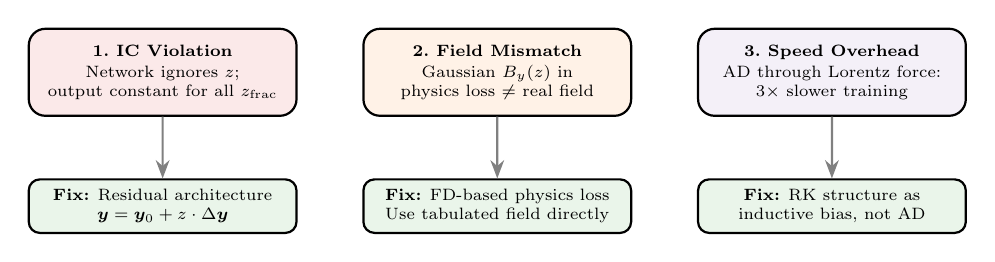
\begin{tikzpicture}[scale=0.85, every node/.style={transform shape},
    prob/.style={draw, thick, rounded corners=6pt, minimum width=4cm, minimum height=1.3cm,
                 align=center, font=\scriptsize},
    fix/.style={draw, thick, rounded corners=4pt, minimum width=4cm, minimum height=0.8cm,
                align=center, font=\scriptsize, fill=nngreen!10},
    arrow/.style={-Stealth, thick, gray}
  ]
    \node[prob, fill=rk4red!10] (p1) at (0,0)
      {\textbf{1.\ IC Violation}\\[1pt]
       Network ignores $z$;\\
       output constant for all $z_\text{frac}$};
    \node[prob, fill=rkorange!10] (p2) at (5,0)
      {\textbf{2.\ Field Mismatch}\\[1pt]
       Gaussian $B_y(z)$ in\\
       physics loss $\neq$ real field};
    \node[prob, fill=physpurple!10] (p3) at (10,0)
      {\textbf{3.\ Speed Overhead}\\[1pt]
       AD through Lorentz force:\\
       $3{\times}$ slower training};

    \node[fix] (f1) at (0,-2)
      {\textbf{Fix:} Residual architecture\\
       $\vb{y} = \vb{y}_0 + z\cdot\Delta\vb{y}$};
    \node[fix] (f2) at (5,-2)
      {\textbf{Fix:} FD-based physics loss\\
       Use tabulated field directly};
    \node[fix] (f3) at (10,-2)
      {\textbf{Fix:} RK structure as\\
       inductive bias, not AD};

    \draw[arrow] (p1) -- (f1);
    \draw[arrow] (p2) -- (f2);
    \draw[arrow] (p3) -- (f3);
  \end{tikzpicture}

  \medskip
  \textcolor{lhcbblue}{\textbf{The RK-PINN architecture addresses all three.}}
\end{frame}

% =============================================================================
\section{The RK-PINN Idea}
% =============================================================================

\begin{frame}{From RK4 to RK-PINN: The Classical Update}
  Given $\frac{d\vb{y}}{dz} = \vb{f}(\vb{y}, z)$, the classical RK4 method advances from $z_n$ to $z_n + h$:
  \begin{columns}[T]
    \column{0.48\textwidth}
    \textbf{Four stage evaluations:}
    \begin{align*}
      \vb{k}_1 &= h\,\vb{f}(\vb{y}_n,\; z_n) \\
      \vb{k}_2 &= h\,\vb{f}\!\left(\vb{y}_n + \tfrac{1}{2}\vb{k}_1,\; z_n + \tfrac{h}{2}\right) \\
      \vb{k}_3 &= h\,\vb{f}\!\left(\vb{y}_n + \tfrac{1}{2}\vb{k}_2,\; z_n + \tfrac{h}{2}\right) \\
      \vb{k}_4 &= h\,\vb{f}\!\left(\vb{y}_n + \vb{k}_3,\; z_n + h\right)
    \end{align*}

    \column{0.48\textwidth}
    \textbf{Weighted combination:}
    \[
      \vb{y}_{n+1} = \vb{y}_n + \tfrac{1}{6}\vb{k}_1 + \tfrac{1}{3}\vb{k}_2 + \tfrac{1}{3}\vb{k}_3 + \tfrac{1}{6}\vb{k}_4
    \]

    \textbf{Key structural observations:}
    \begin{itemize}
      \item Each $\vb{k}_i$ = state increment at a $z$-fraction
      \item Output = initial state + weighted sum
      \item Weights $[\tfrac{1}{6}, \tfrac{1}{3}, \tfrac{1}{3}, \tfrac{1}{6}]$ from Butcher tableau
    \end{itemize}
  \end{columns}

  \medskip
  \centering
  \fbox{\parbox{0.75\textwidth}{\centering
    \textbf{Insight:} This structure --- initial state plus a weighted sum of increments at
    intermediate points --- can be \emph{directly encoded} as a neural network architecture.
  }}
\end{frame}

% -----------------------------------------------------------------------------
\begin{frame}{From RK4 to RK-PINN: The Neural Analogue}
  Replace the analytic derivative $\vb{f}(\vb{y}, z)$ with learned stage increments:
  \begin{columns}[T]
    \column{0.48\textwidth}
    \textbf{Shared feature extraction:}
    \[
      \vb{h} = \text{Backbone}(\vb{x}_0, q/p, \Delta z)
    \]
    \textbf{Per-stage predictions:}
    \[
      \Delta\vb{s}_k = \text{Head}_k(\vb{h},\; z_k), \quad k = 1,\ldots,4
    \]
    where $z_k = z_0 + c_k \cdot \Delta z$, \; $c_k \in \{\tfrac{1}{4}, \tfrac{1}{2}, \tfrac{3}{4}, 1\}$.

    \column{0.48\textwidth}
    \textbf{Learnable RK combination:}
    \[
      \hat{\vb{y}} = \vb{y}_0 + \sum_{k=1}^{4} w_k\,\Delta\vb{s}_k
    \]
    $w_k = \text{softmax}(\alpha_k)$, initialised to $[\tfrac{1}{6}, \tfrac{1}{3}, \tfrac{1}{3}, \tfrac{1}{6}]$.
    \begin{itemize}
      \item Starts as RK4; free to deviate during training
      \item Skip connection $\vb{y}_0 \to$ output guarantees IC
    \end{itemize}
  \end{columns}

  \medskip
  \centering
  \fbox{\parbox{0.85\textwidth}{\centering
    The RK-PINN \textbf{preserves the RK4 decomposition} but replaces numerical derivative
    evaluations with learned functions sharing a common backbone.
  }}
\end{frame}

% -----------------------------------------------------------------------------
\begin{frame}{RK-PINN Architecture Diagram}
  \centering
  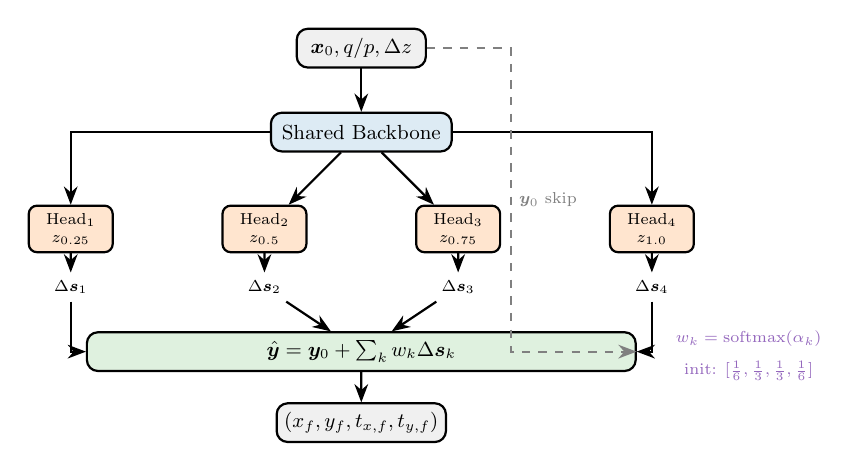
\begin{tikzpicture}[scale=0.82, every node/.style={transform shape},
    box/.style={draw, thick, rounded corners, minimum width=2cm, minimum height=0.6cm,
                align=center, font=\small},
    head/.style={draw, thick, rounded corners=3pt, minimum width=1.3cm, minimum height=0.55cm,
                 align=center, font=\scriptsize},
    arrow/.style={-Stealth, thick},
    darrow/.style={-Stealth, thick, dashed, gray}
  ]
    % Input
    \node[box, fill=lightgray] (input) at (0,0) {$\vb{x}_0, q/p, \Delta z$};

    % Backbone
    \node[box, fill=lhcbblue!15, minimum width=2.8cm] (bb) at (0,-1.3)
      {Shared Backbone};

    % Stage heads
    \node[head, fill=rkorange!20] (h1) at (-4.5,-2.8) {Head$_1$\\$z_{0.25}$};
    \node[head, fill=rkorange!20] (h2) at (-1.5,-2.8) {Head$_2$\\$z_{0.5}$};
    \node[head, fill=rkorange!20] (h3) at (1.5,-2.8) {Head$_3$\\$z_{0.75}$};
    \node[head, fill=rkorange!20] (h4) at (4.5,-2.8) {Head$_4$\\$z_{1.0}$};

    % Stage outputs
    \node[font=\scriptsize] (ds1) at (-4.5,-3.7) {$\Delta\vb{s}_1$};
    \node[font=\scriptsize] (ds2) at (-1.5,-3.7) {$\Delta\vb{s}_2$};
    \node[font=\scriptsize] (ds3) at (1.5,-3.7) {$\Delta\vb{s}_3$};
    \node[font=\scriptsize] (ds4) at (4.5,-3.7) {$\Delta\vb{s}_4$};

    % Weights
    \node[box, fill=nngreen!15, minimum width=8.5cm] (comb) at (0,-4.7)
      {$\hat{\vb{y}} = \vb{y}_0 + \sum_k w_k \Delta\vb{s}_k$};

    % Output
    \node[box, fill=lightgray] (out) at (0,-5.8)
      {$(x_f, y_f, t_{x,f}, t_{y,f})$};

    % Weights label
    \node[font=\scriptsize, physpurple] at (6,-4.5)
      {$w_k = \text{softmax}(\alpha_k)$};
    \node[font=\scriptsize, physpurple] at (6,-5.0)
      {init: $[\frac{1}{6}, \frac{1}{3}, \frac{1}{3}, \frac{1}{6}]$};

    % Arrows
    \draw[arrow] (input) -- (bb);
    \draw[arrow] (bb) -| (h1);
    \draw[arrow] (bb) -- (h2);
    \draw[arrow] (bb) -- (h3);
    \draw[arrow] (bb) -| (h4);
    \draw[arrow] (h1) -- (ds1);
    \draw[arrow] (h2) -- (ds2);
    \draw[arrow] (h3) -- (ds3);
    \draw[arrow] (h4) -- (ds4);
    \draw[arrow] (ds1) |- (comb);
    \draw[arrow] (ds2) -- (comb);
    \draw[arrow] (ds3) -- (comb);
    \draw[arrow] (ds4) |- (comb);
    \draw[arrow] (comb) -- (out);

    % IC line
    \draw[darrow] (input.east) -- ++(1.3,0) |- node[right, pos=0.25, font=\scriptsize, gray] {$\vb{y}_0$ skip} (comb.east);
  \end{tikzpicture}
\end{frame}

% -----------------------------------------------------------------------------
\begin{frame}{Why RK Structure Helps Speed}
  \begin{columns}[T]
    \column{0.48\textwidth}
    \textbf{C++ RK4 (CashKarp):}
    \begin{itemize}\setlength{\itemsep}{1pt}
      \item 6-stage adaptive scheme
      \item $\Delta z = 8000$\,mm, step\,=\,5\,mm
      \item 1600 sub-steps $\times$ 6 = \textbf{9600 field evals}
      \item Each: trilinear lookup in $81^2 \times 146$ grid
      \item Cost: \textbf{7.50\,$\mu$s}
    \end{itemize}

    \medskip
    \textbf{Pure MLP:} single forward pass, no field lookups.\\
    Cost: \textbf{0.83--2.17\,$\mu$s}. Learns mapping as black box.

    \column{0.48\textwidth}
    \textbf{RK-PINN:}
    \begin{itemize}\setlength{\itemsep}{1pt}
      \item 4 stage heads (parallel-capable)
      \item Shared backbone: computed \textbf{once}
      \item \textbf{No field lookups at inference}
      \item Physics encoded in \emph{structure} not loss
    \end{itemize}

    \begin{block}{Speed comparison}
      \centering\small
      \begin{tabular}{lr}
        \toprule
        \textbf{Method} & \textbf{Field evals} \\
        \midrule
        C++ CashKarp & 9600 \\
        PINN (10 collocation) & 10 \textit{(train only)} \\
        RK-PINN / MLP & \textbf{0} \\
        \bottomrule
      \end{tabular}
    \end{block}
  \end{columns}
\end{frame}

% =============================================================================
\section{The Residual Architecture}
% =============================================================================

\begin{frame}{Residual Architecture --- Guaranteeing Initial Conditions}
  \begin{columns}[T]
    \column{0.46\textwidth}
    \textbf{Constraint:} at $z{=}z_0$, $\hat{\vb{y}}(z_0) = \vb{y}_0$.

    \smallskip
    {\small\textbf{Na\"ive:} $\hat{\vb{y}} = \text{NN}(\vb{x}_0, q/p, \Delta z)$
    --- no $z_f$, IC not enforced. \textcolor{rk4red}{\ding{55}}}

    \smallskip
    {\small\textbf{Residual:} parameterise \emph{deviation}:
    $\hat{\vb{y}}(z) = \vb{y}_0 + z_f \cdot \Delta\vb{y}_\text{NN}$}

    \smallskip
    {\small $z_f{=}0 \!\Rightarrow\! \hat{\vb{y}}{=}\vb{y}_0$ \textcolor{nngreen}{\ding{51}};\;
    $z_f{=}1 \!\Rightarrow\!$ full correction.}

    \vspace{4pt}
    \begin{alertblock}{Impact}
      \centering\footnotesize
      \begin{tabular}{lcc}
        \toprule
        & \textbf{Na\"ive} & \textbf{Residual} \\
        \midrule
        IC err.\ & 2758\,mm & \textbf{0.0\,mm} \\
        Pos.~err.\ & 593\,mm & 28\,$\mu$m \\
        \bottomrule
      \end{tabular}
    \end{alertblock}

    \column{0.50\textwidth}
    \textbf{Explicit form} ($z_f \equiv z_\text{frac}$):

    {\small\textit{Positions} (straight-line + deflection):}
    \vspace{-6pt}
    {\small\begin{align*}
      \hat{x} &= x_0 + t_{x,0}\Delta z\,z_f + z_f\cdot\delta x_\text{NN} \\
      \hat{y} &= y_0 + t_{y,0}\Delta z\,z_f + z_f\cdot\delta y_\text{NN}
    \end{align*}}
    \vspace{-12pt}

    {\small\textit{Slopes} (constant + curvature):}
    \vspace{-6pt}
    {\small\begin{align*}
      \hat{t}_x &= t_{x,0} + z_f\cdot\delta t_{x,\text{NN}} \\
      \hat{t}_y &= t_{y,0} + z_f\cdot\delta t_{y,\text{NN}}
    \end{align*}}
    \vspace{-10pt}

    {\small Network outputs 4 corrections $(\delta x, \delta y, \delta t_x, \delta t_y)$; residual skip connection \textbf{guarantees} $\hat{\vb{y}}(z_0) = \vb{y}_0$.}
  \end{columns}
\end{frame}

% =============================================================================
\section{Literature Solutions}
% =============================================================================

\begin{frame}{Paper 1: Finite Difference PINNs}
  \textit{``Physics-informed deep learning based on the finite difference method''}

  \begin{columns}[T]
    \column{0.55\textwidth}
    \textbf{Core idea:} Replace AD with finite differences for the physics loss.
    \[
      \frac{\partial \hat{u}}{\partial z}\bigg|_{z_i} \approx \frac{\hat{u}(z_i + \delta) - \hat{u}(z_i - \delta)}{2\delta}
    \]

    \textbf{Why this matters for us:}
    \begin{enumerate}\setlength{\itemsep}{1pt}
      \item AD needs differentiable field $\Rightarrow$ forced Gaussian
      \item FD only needs evaluations $\Rightarrow$ use \texttt{twodip.rtf}
      \item No computational graph $\Rightarrow$ lower memory
      \item FD $\approx$ MLP training speed (vs.\ $3\times$ for AD)
    \end{enumerate}

    \column{0.42\textwidth}
    \begin{block}{Field model comparison}
      \centering\small
      \begin{tabular}{lcc}
        \toprule
        & \textbf{AD} & \textbf{FD} \\
        \midrule
        Differentiable? & Required & Not needed \\
        Field model & Gaussian & Any \\
        Mismatch & 3.2\% & \textbf{0\%} \\
        Memory & High & Low \\
        Speed & $3\times$ MLP & ${\sim}1.2\times$ \\
        \bottomrule
      \end{tabular}
    \end{block}

    \begin{exampleblock}{For RK-PINN}
      FD physics loss at each RK stage with the real field map = \textbf{physically correct} training.
    \end{exampleblock}
  \end{columns}
\end{frame}

% -----------------------------------------------------------------------------
\begin{frame}{Paper 2: Data-Free PINNs}
  \textit{Misyris et al.\ --- ``Learning without Data,'' IEEE SmartGridComm (2021)}

  \begin{columns}[T]
    \column{0.55\textwidth}
    \textbf{Core idea:} Train with \textbf{zero data}, physics loss only.
    \[
      \mathcal{L} = \lambda_\text{PDE}\,\mathcal{L}_\text{PDE} + \lambda_\text{IC}\,\mathcal{L}_\text{IC}
    \]

    \textbf{Their result:}
    \begin{itemize}\setlength{\itemsep}{1pt}
      \item Solved power grid DAE system (no data)
      \item Orders-of-magnitude speedup
      \item Generalises across IC families
    \end{itemize}

    \textbf{For us:}
    \begin{itemize}\setlength{\itemsep}{1pt}
      \item Pure data-free unlikely (6D, complex field)
      \item \textbf{Hybrid:} 1--5M samples + physics loss
    \end{itemize}

    \column{0.42\textwidth}
    \begin{block}{Data requirements}
      \centering\small
      \begin{tabular}{lcc}
        \toprule
        & \textbf{Initial} & \textbf{Hybrid} \\
        \midrule
        Training data & 50M & 1--5M \\
        Gen.\ time & Hours & Minutes \\
        Physics loss & Broken & Correct \\
        \bottomrule
      \end{tabular}
    \end{block}

    \begin{alertblock}{Speed implication}
      Less training data $\Rightarrow$ faster iteration cycles.\\
      Physics loss compensates for reduced data coverage.
    \end{alertblock}
  \end{columns}
\end{frame}

% -----------------------------------------------------------------------------
\begin{frame}{Paper 3: Temporal Domain Decomposition with DeepONets}
  \textit{``Long-time integration of parametric evolution equations with physics-informed DeepONets''}

  \begin{columns}[T]
    \column{0.55\textwidth}
    \textbf{Problem:} PINNs fail for long time horizons (spectral bias).

    \textbf{Solution:} Split into short windows, chain predictions.
    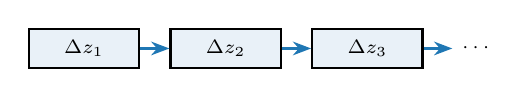
\begin{tikzpicture}[
      win/.style={draw, thick, fill=lhcbblue!10, minimum width=1.4cm, minimum height=0.5cm, font=\scriptsize},
      arrow/.style={-Stealth, thick, lhcbblue}
    ]
      \node[win] (w1) at (0,0) {$\Delta z_1$};
      \node[win] (w2) at (1.8,0) {$\Delta z_2$};
      \node[win] (w3) at (3.6,0) {$\Delta z_3$};
      \node[font=\scriptsize] (dots) at (5,0) {$\cdots$};
      \draw[arrow] (w1) -- (w2);
      \draw[arrow] (w2) -- (w3);
      \draw[arrow] (w3) -- (dots);
    \end{tikzpicture}

    \textbf{Direct relevance:}
    \begin{itemize}\setlength{\itemsep}{1pt}
      \item Initial study: fixed $\Delta z = 8000$\,mm (monolithic)
      \item \textbf{Short-step chaining} (e.g.\ $4 \times 2000$\,mm) enables variable step sizes
      \item Compatible with Kalman filter (sequential)
    \end{itemize}

    \column{0.42\textwidth}
    \begin{exampleblock}{Speed estimate}
      \begin{itemize}\setlength{\itemsep}{1pt}
        \item Model for $\Delta z = 2000$\,mm
        \item $\sim$0.5\,$\mu$s/step $\times$ 4 = 2.0\,$\mu$s
        \item Still $\leq$ C++ RK4 (7.50\,$\mu$s)
      \end{itemize}
    \end{exampleblock}

    \begin{block}{Operator learning}
      DeepONet learns the \emph{solution operator}:
      $\mathcal{G}: \vb{s}_0 \mapsto \vb{s}(\Delta z)$.
      One network, all initial states \& momenta.
    \end{block}
  \end{columns}
\end{frame}

% -----------------------------------------------------------------------------
\begin{frame}{Paper 4: RK-PINNs in the Literature}
  \textit{``Parameter estimation and modeling of nonlinear dynamical systems based on RK-PINN''}

  \begin{columns}[T]
    \column{0.48\textwidth}
    \textbf{Literature RK-PINN:}
    \begin{itemize}\setlength{\itemsep}{1pt}
      \item Multi-stage with Butcher tableau weights
      \item \textbf{Full PDE residual} at each stage
      \item IC satisfaction via residual form
      \item Forward + inverse problems
    \end{itemize}

    \smallskip
    \textbf{vs.\ our initial RK-PINN:}
    \begin{itemize}\setlength{\itemsep}{1pt}
      \item[\textcolor{rk4red}{\ding{55}}] IC not guaranteed
      \item[\textcolor{rk4red}{\ding{55}}] Gaussian field in physics loss
      \item[\textcolor{nngreen}{\ding{51}}] Learnable softmax weights
      \item[\textcolor{nngreen}{\ding{51}}] Shared backbone
    \end{itemize}

    \column{0.48\textwidth}
    \begin{alertblock}{Inverse problem capability}
      RK-PINN could \textbf{simultaneously}:
      \begin{enumerate}\setlength{\itemsep}{1pt}
        \item Predict trajectory (forward)
        \item Estimate $q/p$ (inverse)
        \item Refine field map (calibration)
      \end{enumerate}
    \end{alertblock}

    \begin{block}{What we need to fix}
      \begin{enumerate}\setlength{\itemsep}{1pt}
        \item Residual PINN formulation
        \item Full Lorentz residual at each stage
        \item FD-based physics loss (real field)
      \end{enumerate}
    \end{block}
  \end{columns}
\end{frame}

% =============================================================================
\section{The Combined Strategy}
% =============================================================================

\begin{frame}{Putting It Together: Residual RK-PINN}
  \centering
  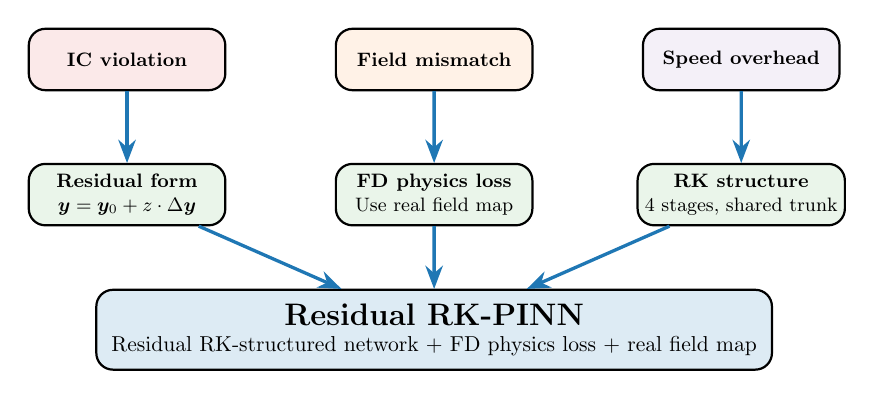
\begin{tikzpicture}[scale=0.78, every node/.style={transform shape},
    comp/.style={draw, thick, rounded corners=6pt, minimum width=3.2cm, minimum height=1cm,
                 align=center, font=\small},
    arrow/.style={-Stealth, very thick, lhcbblue}
  ]
    % Top row: problems
    \node[comp, fill=rk4red!10] (ic) at (0,2.2) {\textbf{IC violation}};
    \node[comp, fill=rkorange!10] (field) at (5,2.2) {\textbf{Field mismatch}};
    \node[comp, fill=physpurple!10] (speed) at (10,2.2) {\textbf{Speed overhead}};

    % Middle: solutions
    \node[comp, fill=nngreen!10] (res) at (0,0) {\textbf{Residual form}\\$\vb{y} = \vb{y}_0 + z\cdot\Delta\vb{y}$};
    \node[comp, fill=nngreen!10] (fd) at (5,0) {\textbf{FD physics loss}\\Use real field map};
    \node[comp, fill=nngreen!10] (rk) at (10,0) {\textbf{RK structure}\\4 stages, shared trunk};

    % Bottom: combined
    \node[comp, fill=lhcbblue!15, minimum width=11cm, minimum height=1.3cm] (rkv3) at (5,-2.2)
      {\Large\textbf{Residual RK-PINN}\\[1pt]
       \normalsize Residual RK-structured network + FD physics loss + real field map};

    % Arrows
    \draw[arrow] (ic) -- (res);
    \draw[arrow] (field) -- (fd);
    \draw[arrow] (speed) -- (rk);
    \draw[arrow] (res) -- (rkv3);
    \draw[arrow] (fd) -- (rkv3);
    \draw[arrow] (rk) -- (rkv3);
  \end{tikzpicture}
\end{frame}

% -----------------------------------------------------------------------------
\begin{frame}{Speed-Accuracy Trade-off: Target Region}
  \begin{columns}[T]
    \column{0.55\textwidth}
    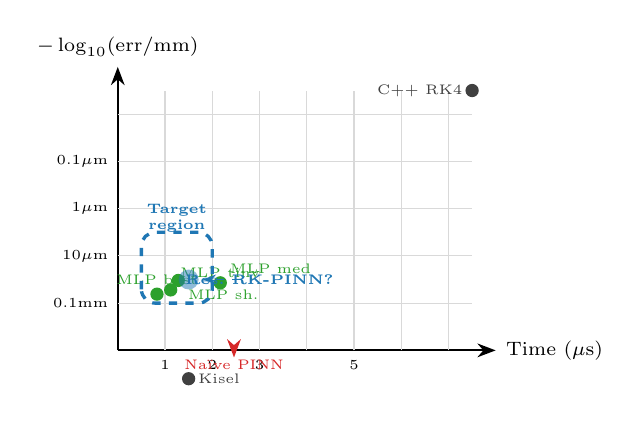
\begin{tikzpicture}[scale=0.60]
      % Axes
      \draw[-Stealth, thick] (0,0) -- (8,0) node[right] {\scriptsize Time ($\mu$s)};
      \draw[-Stealth, thick] (0,0) -- (0,6) node[above] {\scriptsize$-\log_{10}$(err/mm)};
      % Grid
      \foreach \y in {1,...,5} {
        \draw[gray!30] (0,\y) -- (7.5,\y);
      }
      \foreach \x in {1,...,7} {
        \draw[gray!30] (\x,0) -- (\x,5.5);
      }
      % Axis labels
      \node[below, font=\tiny] at (1,0) {1};
      \node[below, font=\tiny] at (2,0) {2};
      \node[below, font=\tiny] at (3,0) {3};
      \node[below, font=\tiny] at (5,0) {5};
      \node[left, font=\tiny] at (0,1) {0.1mm};
      \node[left, font=\tiny] at (0,2) {10$\mu$m};
      \node[left, font=\tiny] at (0,3) {1$\mu$m};
      \node[left, font=\tiny] at (0,4) {0.1$\mu$m};

      % Data points
      % MLP tiny: 1.12 us, 53 um -> (1.12, ~1.3)
      \fill[nngreen] (1.12, 1.28) circle (4pt) node[above right, font=\tiny] {MLP tiny};
      % MLP v2 single: 0.83 us, 65 um
      \fill[nngreen] (0.83, 1.19) circle (4pt) node[above, font=\tiny] {MLP best};
      % MLP medium: 2.17 us, 37 um
      \fill[nngreen] (2.17, 1.43) circle (4pt) node[above right, font=\tiny] {MLP med};
      % MLP shallow: 1.28, 33 um
      \fill[nngreen] (1.28, 1.48) circle (4pt) node[below right, font=\tiny] {MLP sh.};
      % C++ RK4: 7.50, ref (0 error, plot at top)
      \fill[darkgray] (7.50, 5.5) circle (4pt) node[left, font=\tiny] {C++ RK4};
      % Kisel: 1.50, 39800 um -> very low
      \fill[darkgray] (1.50, -0.6) circle (4pt) node[right, font=\tiny] {Kisel};
      % V1 PINN: 2.46, 593mm -> off chart bottom
      \node[rk4red, font=\tiny] at (2.46, -0.3) {Na\"ive PINN};
      \draw[rk4red, thick, -Stealth] (2.46, 0.1) -- (2.46, -0.15);

      % Target region
      \draw[lhcbblue, very thick, dashed, rounded corners=5pt]
        (0.5, 1.0) rectangle (2.0, 2.5);
      \node[lhcbblue, font=\tiny\bfseries, align=center] at (1.25, 2.8) {Target\\region};

      % RK-PINN v3 target
      \fill[lhcbblue, opacity=0.5] (1.5, 1.5) circle (6pt);
      \node[lhcbblue, font=\tiny\bfseries] at (3.0, 1.5) {Res.\ RK-PINN?};
      \draw[lhcbblue, dashed, -Stealth] (2.6, 1.5) -- (1.8, 1.5);
    \end{tikzpicture}

    \column{0.40\textwidth}
    \begin{block}{Target specs}
      \begin{itemize}\setlength{\itemsep}{1pt}
        \item Inference: $\leq 2.0$\,$\mu$s
        \item Accuracy: $\leq 100$\,$\mu$m
        \item Physics-consistent trajectories
        \item Variable $\Delta z$ support
      \end{itemize}
    \end{block}

    \begin{exampleblock}{Expected performance}
      \begin{itemize}\setlength{\itemsep}{1pt}
        \item RK-PINN \textit{med}: 5.59\,$\mu$s
        \item Backbone shared, stage heads differ
        \item \textbf{Tiny:} $\sim$1.5--2.0\,$\mu$s
        \item Physics $\Rightarrow$ better accuracy/param
      \end{itemize}
    \end{exampleblock}
  \end{columns}
\end{frame}

% =============================================================================
\section{Roadmap}
% =============================================================================

\begin{frame}{Implementation Priority}
  \begin{enumerate}\setlength{\itemsep}{4pt}
    \item[\textcolor{rk4red}{\textbf{P1}}] \textbf{Residual architecture fix} --- prerequisite for everything
      \begin{itemize}\setlength{\itemsep}{0pt}
        \item $\vb{y}(z) = \vb{y}_0 + z_\text{frac}\cdot\text{MLP}(\cdots)$; guarantees IC by construction
      \end{itemize}

    \item[\textcolor{rkorange}{\textbf{P2}}] \textbf{FD-based physics loss} with real field map
      \begin{itemize}\setlength{\itemsep}{0pt}
        \item Replace AD with $(\hat{u}(z{+}\delta) - \hat{u}(z{-}\delta))/2\delta$; use \texttt{twodip.rtf} directly
        \item Training speed: $\sim$MLP speed (vs.\ $3\times$ for AD)
      \end{itemize}

    \item[\textcolor{lhcbblue}{\textbf{P3}}] \textbf{Residual RK-PINN} with short-step chaining
      \begin{itemize}\setlength{\itemsep}{0pt}
        \item Train on $\Delta z = 1000$--$2000$\,mm; chain 4--8 steps
        \item $\sim$0.5\,$\mu$s/step; total 2--4\,$\mu$s (competitive with C++)
      \end{itemize}

    \item[\textcolor{nngreen}{\textbf{P4}}] \textbf{Inverse mode} --- exploratory
      \begin{itemize}\setlength{\itemsep}{0pt}
        \item Estimate $q/p$ from track hits; field map calibration
      \end{itemize}
  \end{enumerate}
\end{frame}

% =============================================================================
\section{Summary}
% =============================================================================

\begin{frame}{Summary}
  \begin{enumerate}\setlength{\itemsep}{3pt}
    \item \textbf{The problem is well-suited for RK-PINNs:}
      \begin{itemize}\setlength{\itemsep}{0pt}
        \item Lorentz force ODEs have RK4 integration as natural structure
        \item Field is smooth, slowly varying, tabulated on regular grid
        \item Speed critical: 9600 field evaluations $\to$ single forward pass
      \end{itemize}

    \item \textbf{Initial failures were architectural, not fundamental:}
      \begin{itemize}\setlength{\itemsep}{0pt}
        \item IC violation $\to$ residual fix; field mismatch $\to$ FD physics loss
        \item Literature confirms: PINNs fail on complex ODEs unless carefully designed
      \end{itemize}

    \item \textbf{Literature provides a clear path:}
      \begin{itemize}\setlength{\itemsep}{0pt}
        \item FD-PINNs, domain decomposition, RK-structure, inverse capability
      \end{itemize}

    \item \textbf{Target:} Residual RK-PINN at $\leq 2$\,$\mu$s, $\leq 100$\,$\mu$m accuracy,
          physics-consistent trajectories.
  \end{enumerate}
\end{frame}

% =============================================================================
\begin{frame}[allowframebreaks]{References}
  \small
  \begin{thebibliography}{10}
    \bibitem{Raissi2019}
    M.~Raissi, P.~Perdikaris, G.E.~Karniadakis,
    ``Physics-informed neural networks,''
    \textit{J.~Comput.~Phys.} \textbf{378}, 686 (2019).

    \bibitem{FD-PINN}
    ``Physics-informed deep learning based on the finite difference method for efficient and accurate numerical solution of PDEs.''

    \bibitem{DataFree}
    G.S.~Misyris, A.~Stiasny, S.~Chatzivasileiadis,
    ``Learning without Data: PINNs for Fast Time-Domain Simulation,''
    \textit{IEEE SmartGridComm} (2021).

    \bibitem{DeepONet-LT}
    ``Long-time integration of parametric evolution equations with physics-informed DeepONets.''

    \bibitem{RK-PINN}
    ``Parameter estimation and modeling of nonlinear dynamical systems based on RK-PINN.''

    \bibitem{Krishnapriyan2021}
    A.S.~Krishnapriyan et al.,
    ``Characterizing possible failure modes in PINNs,''
    \textit{NeurIPS} (2021).

    \bibitem{DeepONet}
    L.~Lu, P.~Jin, G.E.~Karniadakis,
    ``DeepONet: Learning nonlinear operators,''
    \textit{Nature Mach.~Intell.} \textbf{3}, 218 (2021).

    \bibitem{FNO}
    Z.~Li et al.,
    ``Fourier Neural Operator for Parametric PDEs,''
    \textit{ICLR} (2021).
  \end{thebibliography}
\end{frame}

% =============================================================================
\begin{frame}[plain]
  \centering
  \vfill
  {\Huge\textcolor{lhcbblue}{Thank you}}

  \bigskip
  {\large Questions?}

  \bigskip
  \small
  \texttt{George.Scriven@uhasselt.be} \\
  \texttt{George.William.Scriven@cern.ch}
  \vfill
\end{frame}

\end{document}
